\documentclass[border=10pt]{standalone}
\usepackage{tikz}
\begin{document}
\noindent
\begin{minipage}{.35\textwidth}
    \centering
    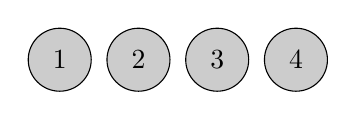
\begin{tikzpicture}[<-,sibling distance=6em,
        every node/.style = {shape=circle, rounded corners,
            draw, align=center,minimum size=0.8cm,
        fill=black!20}]]
        \node (1) at (0, 0) {1};
        \node (2) at (1, 0) {2};
        \node (3) at (2, 0) {3};
        \node (4) at (3, 0) {4};
    \end{tikzpicture}
\end{minipage}
\begin{minipage}{.05\textwidth}
    \centering
    $\Longrightarrow$
\end{minipage}
\begin{minipage}{.28\textwidth}
    \centering
    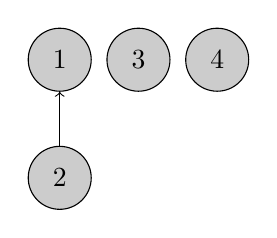
\begin{tikzpicture}[<-,sibling distance=6em,
        every node/.style = {shape=circle, rounded corners,
            draw, align=center,minimum size=0.8cm,
        fill=black!20}]]
        \node (1) at (0, 0) {1}
            child {node {2}};
        \node (3) at (1, 0) {3};
        \node (4) at (2, 0) {4};
    \end{tikzpicture}
\end{minipage}
\begin{minipage}{.05\textwidth}
    \centering
    $\Longrightarrow$
\end{minipage}
\begin{minipage}{.2\textwidth}
    \centering
    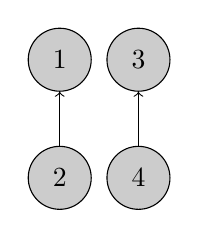
\begin{tikzpicture}[<-,sibling distance=6em,
        every node/.style = {shape=circle, rounded corners,
            draw, align=center,minimum size=0.8cm,
        fill=black!20}]]
        \node at (0, 0) {1}
            child {node {2}};
        \node at (1, 0) {3}
            child {node {4}};
    \end{tikzpicture}
\end{minipage}
\begin{minipage}{.05\textwidth}
    \centering
    $\Longrightarrow$
\end{minipage}
\begin{minipage}{.2\textwidth}
    \centering
    \begin{tikzpicture}[<-,sibling distance=3em,
        every node/.style = {shape=circle, rounded corners,
            draw, align=center,minimum size=0.8cm,
        fill=black!20}]]
        \node at (0, 0) {1}
            child {node {2}}
            child {node {3}
                child {node {4}}};
        };
    \end{tikzpicture}
\end{minipage}
\end{document}
